\chapter{Testing}\label{cha:testing}

% Covers unit tests, and performance tests

As discussed in Chapter \ref{cha:intro}, the high level aim of this system is to improve the speed of data processing for large datasets. Therefore, it is important to conduct performance testing of the overall system. This section aims to cover a number of methods in which the performance of the completed solution is evaluated.

Firstly, raw performance testing is conducted against a typical data processing solution, Microsoft SQL Server. Then, a number of alternative approaches are assessed for determining how well the cluster leverages the parallelisation of running the computation over multiple nodes. This includes

\section{Unit Tests}
Thorough unit testing is important for any software engineering focused project. By writing tests throughout development, the expected behaviour of individual components in the system can be validated. Through the use of continuous integration/continuous deployment (CI/CD) pipelines, this behaviour can continue to be validated as other parts of the system are improved, to ensure changes do not break the behaviour of the component. 

Scalatest was chosen as the unit test framework \todo{reference}. Furthermore, both gRPC and Akka Actors provide classes for writing unit tests around the frameworks, and this is combined with Mockito to mock any dependencies that cannot be run during testing - for example, Cassandra \todo{reference}. Using these tools and frameworks, unit tests have been written for the majority of core code; this includes the DSL, query model and partitioning code among other classes. In total, more than 350 individual tests were written for this project, split across the Python frontend, core code, orchestrator and worker code.

\section{Test Data}
To conduct the performance testing, fake data is created to test the different operations of the system. As the intended users of this system are of a financial background, fake loan origination (loan creation) data is generated. This uses a short Python script which provides the following data, randomised between specified bounds.
\begin{itemize}
	\item Loan Amount
	\item Loan Duration
	\item Loan Interest Rate
	\item Loan Origination Date
\end{itemize}

Figure \ref{fig:fake-loan-data} shows ten example records of fake loan origination data.

\begin{figure}[h]
	\centering
	\begin{tabular}{| l | l | l | l | l |}
		\hline
		\textbf{Loan ID} & \textbf{Amount} & \textbf{Interest Rate} & \textbf{Duration (Yrs)} & \textbf{Origination Date} \\ \hline 
		0 & 590,418 & 0.041139 & 24 & 2021-04-23 18:13:00   \\ \hline
		1 & 697,824 & 0.095023 & 20 & 2021-10-06 20:07:00    \\ \hline
		2 & 271,853 & 0.029358 & 23 & 2021-03-08 05:12:00    \\ \hline
		3 & 329,950 & 0.038111 & 23 & 2021-01-18 21:05:00    \\ \hline
		4 & 1,381,994 & 0.055411 & 30 & 2021-05-13 15:54:00  \\ \hline
		5 & 1,365,793 & 0.0093872 & 29 & 2021-05-04 03:18:00  \\ \hline
		6 & 1,143,926 & 0.078929 & 21 & 2021-07-11 19:10:00   \\ \hline
		7 & 461,215 & 0.082520 & 23 & 2021-05-04 17:50:00    \\ \hline
		8 & 287,307 & 0.040382 & 21 & 2021-05-20 06:08:00   \\ \hline
		9 & 191,668 & 0.061314 & 25 & 2021-09-03 16:21:00    \\ \hline
	\end{tabular}
	\caption{Example Loan Origination Data}
	\label{fig:fake-loan-data}
\end{figure}

\section{SQL vs Cluster Solution}
This section will compare the performance of an instance of Microsoft SQL Server, against the completed solution, referred to as the Cluster Processor in this testing. 

\paragraph{Test Plan}
The tests are conducted for the three types of query that the cluster processor supports: Select, Filter and Group By. Within each type of query, a simple, and a complex version of the query will be written and tested. For the cluster processor, the tests are run tables containing loan origination data with the following number of rows: 1000, 10000, 100,000, 1 million and 10 million rows. For SQL, tables with the same number of rows are generated, as well as two further tables: 50 million and 100 million rows. These extra tables are not used for the cluster processor due to time and cost constraints.

To reduce the effect of random error, each test is run 5 times, and the results averaged across all tests. This is particularly important when running on a cloud environment, as there is less control over the hardware running the tests. In particular, there is no control over what other work that hardware is doing alongside the testing, so averaging a number of results should reduce any impact this has.

In all of these tests, Microsoft SQL Server was running on an instance of Azure SQL Database \todo{reference}. The Cluster Processor was running on Azure Kubernetes Service, with a pool of three B4ms nodes available \todo{reference}. Each B4ms node has a total of 4 vCores, and 16GB memory, but the actual CPU and memory available to each pod in the cluster is controlled by Kubernetes.

\subsection{Controls}
A number of variables must be considered which could have an impact on the results of this test. The testing attempts to mitigate the effects of these variables in order to make the results as comparable as possible.

\paragraph{CPU and Memory}
CPU and Memory is the largest contributing factor that will affect how quickly the computation is performed, both on SQL, and the Cluster Processor. Ensuring these are comparable is essential for producing reliable test results. For Azure SQL Database, a slider can be used to set the maximum number of vCores available, and a set amount of memory is assigned based on the number of cores. In this case, a maximum of 6 vCores were used, which results in a maximum of 18GB memory accessible to the database.

As the Cluster Processor is running on Kubernetes, completely granular control over the number of vCores and amount of memory available to each node is possible using resource limits enforced by Kubernetes \todo{reference}. Workers were configured to have a maximum of 2 vCores, and 6GB memory available to each, with 3 workers in total. As a result, the cluster as a whole has 6 vCores and 18GB memory available, the same as the SQL database.

\paragraph{Network Latency}
Controlling network latency is particularly important for small requests which resolve quickly. For a request that takes 0.5s to complete, 100ms of latency will make the completion 20\% slower. Testing was always performed on an instance of Azure Cloud Shell \todo{reference}, which is a terminal instance running inside the same Azure datacenter as the SQL server or Cluster Processor. This has the effect of minimising network latency, or at least ensuring it is comparable between both tests.

\paragraph{Warm-Up}
Both SQL and Cluster Processor have a warm-up periods when they are first started. Azure SQL Database is run using a serverless computation style, which means the server is scaled to 0 resources when it is unused. This has the disadvantage that when a query is first run, there is a short delay while the resources are provisioned again. Cluster Processor has a similar warm-up when it is first started, because the gRPC connections between the orchestrator and workers are not actually created until the first request is made. To overcome both of these warm-up periods, a number of queries are run just before testing begins, and the time taken to run these is not tracked.

%prewarm described here: https://learn.microsoft.com/en-us/azure/azure-sql/database/serverless-tier-overview?view=azuresql&tabs=general-purpose


\subsection{Select Query}
The first query is a pure select, which essentially tests how fast both solutions can send results over the network. Figure \ref{fig:sql-select-simple} shows the SQL query, and Figure \ref{fig:cluster-select-simple} shows the Cluster Processor query. The second select query is a more complex select, with some conversion operations to test if this has an impact on the computation time. Figures \ref{fig:sql-select-complex} and \ref{fig:cluster-select-complex} show the queries.

\paragraph{Results} The results for this query are shown in Figure \ref{fig:select-graph}. Data is only available for Cluster Processor up to 100,000 rows because of a memory issue when passing data from the workers to the orchestrator, which is analysed further in Chapter \ref{cha:evaluation}. As a result, the graph is filtered to exclude the SQL results for 50 and 100 million rows.

However, the data that is available shows that the Cluster Processor is more than 10x slower at performing Select queries than SQL. This is most likely related to the format used to send the result data, which requires serialising both the type and value of each cell in the data for transmission. For both SQL and the Cluster Processor, there is no significant difference between the raw Select, and the Select with operations. The largest difference is at 100k rows for Cluster Processor, where there is a 0.3s increase when computing the operations compared to a raw Select.

\begin{figure}[h]
	\centering
	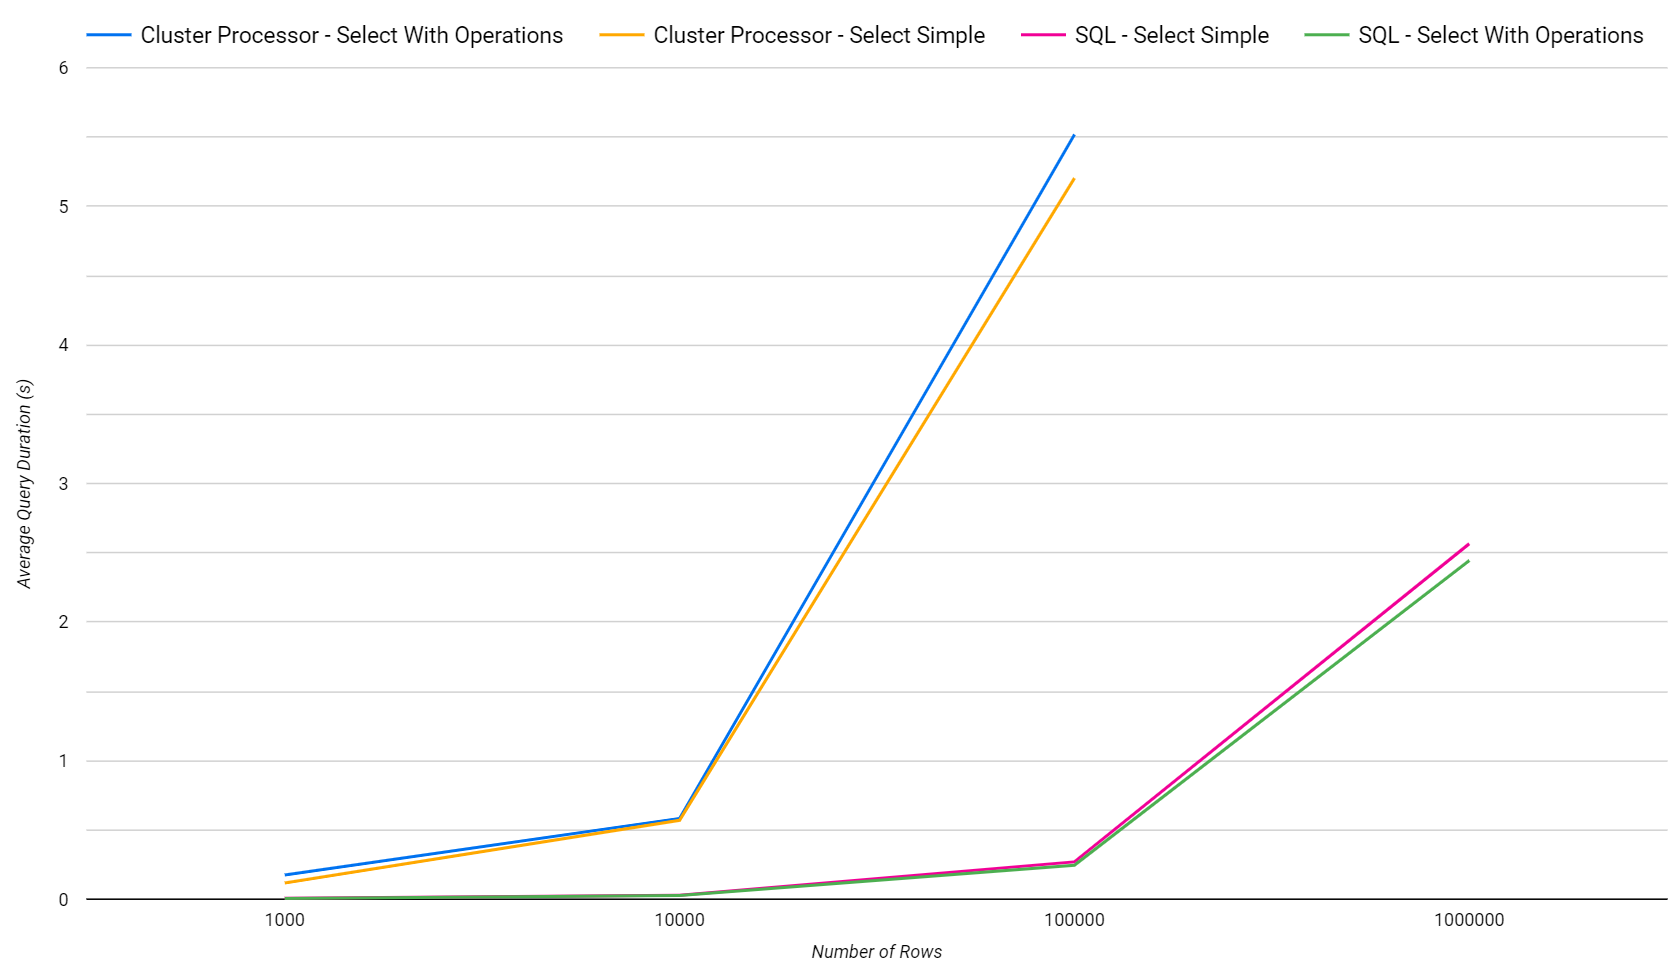
\includegraphics[width=0.8\linewidth]{chapters/diagrams/testing/select-simple-1k-1m}
	\caption{SQL vs Cluster Processor - Select Query Results}
	\label{fig:select-graph}
\end{figure}

\subsection{Filter Query}
The first query is a simple filter, with no AND/OR combinations. Figures \ref{fig:sql-filter-simple} and \ref{fig:cluster-filter-simple} show the queries.  The second filter is more complex, testing both boolean operators. Figures \ref{fig:sql-filter-complex} and \ref{fig:cluster-filter-complex} show the queries.
The results for this query are shown in Figure \ref{fig:filter-graph}. 

\paragraph{Results}
The results for this query are shown in Figure \ref{fig:filter-graph}, where testing was performed for the full range of datasets in both SQL and the Cluster Processor. The results show that SQL is again significantly faster in this test case, producing results around 15-20x faster. This is likely to be partially caused by the transmission format, as with the Select queries. However, it is also likely that SQL is able to exploit caching more extensively over repeated tests when compared to the Cluster Processor, particularly with the smaller tables which can be held in memory permanently. This is because the Cluster Processor fetches fresh data from Cassandra every time the query is called.

Another relevant insight from this data is that the complex filter reliably executes faster than the simple filter across all results. For the Cluster Processor, it is nearly 2 seconds faster on average at 10 million rows, and for SQL it is almost 6 seconds faster at 100 million rows. This is to be expected, since the complex filter is  more restrictive in the results that it returns, so there is less data to transfer over the network.

\begin{figure}[h]
	\centering
	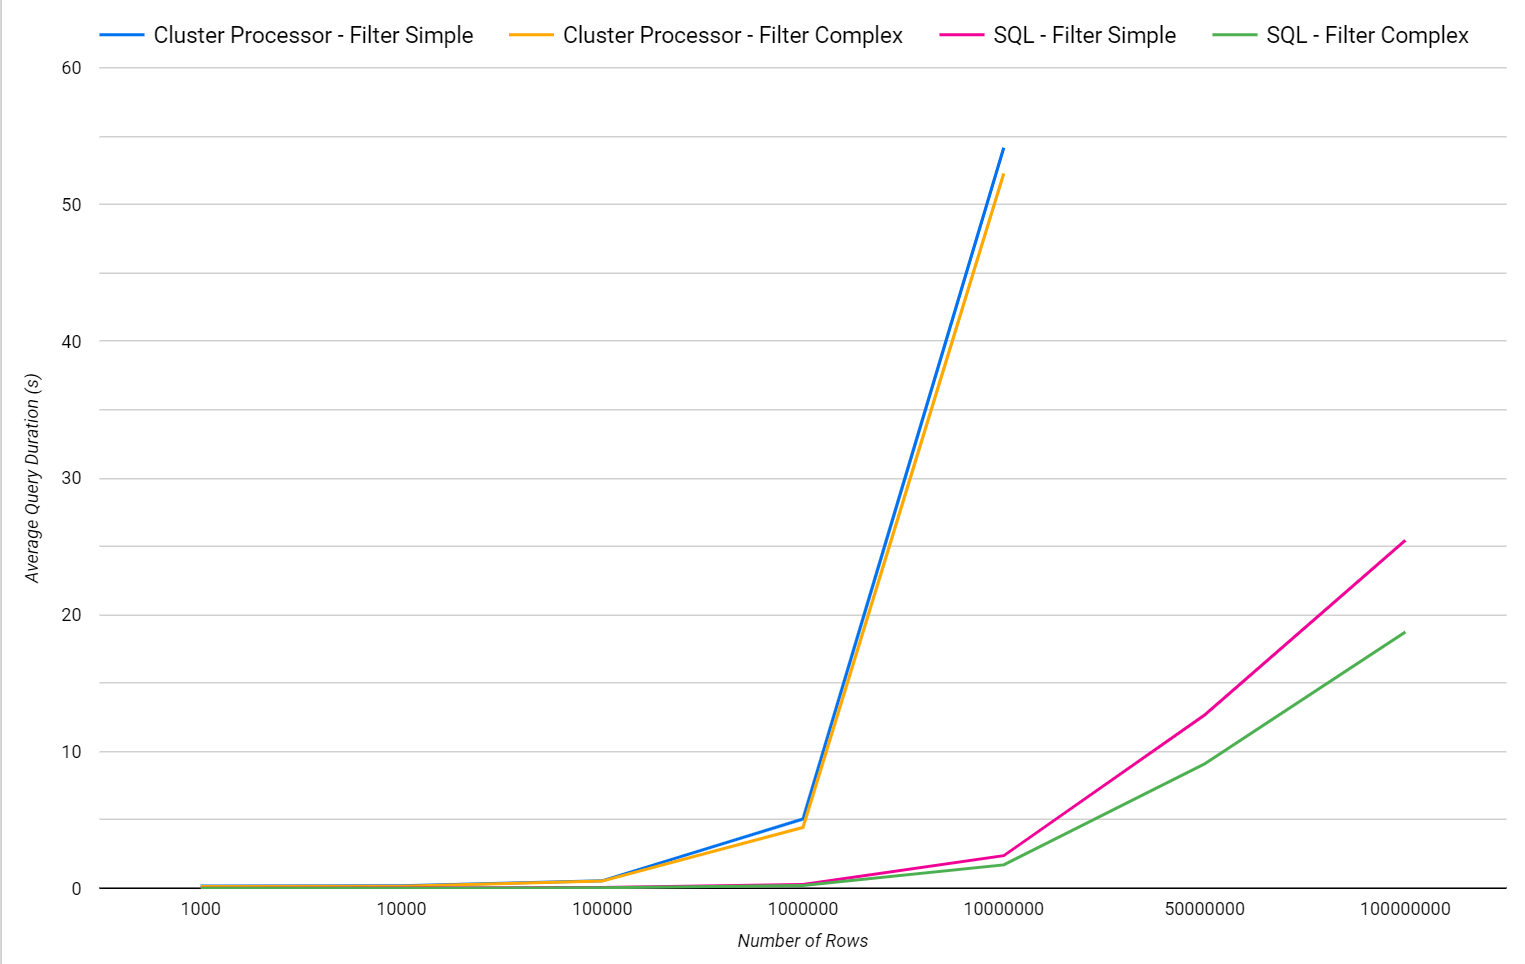
\includegraphics[width=0.8\linewidth]{chapters/diagrams/testing/filter-1k-100m}
	\caption{SQL vs Cluster Processor - Filter Query Results}
	\label{fig:filter-graph}
\end{figure}


\subsection{Group By Query}
The first query is a simple group by, essentially acting as a \texttt{DISTINCT} check. Figures \ref{fig:sql-group-by-simple} and \ref{fig:cluster-group-by-simple} show the queries. The second group by is more complex, featuring a number of aggregations. Figures \ref{fig:sql-group-by-complex} and \ref{fig:cluster-group-by-complex} show the queries. 

\paragraph{Results}
The results for this query are shown in Figure \ref{fig:group-by-graph}, where again testing was performed for the full range of datasets in both solutions. SQL is significantly faster, and scales much better as the data sizes increase. For the Cluster Processor, the aggregate group by is over twice as fast on average than the simple version at 10 million records. The testing was performed sequentially, with no break between tests, so it is unclear why this result is so much faster Furthermore, the same difference in computation time is not present at smaller data volumes. This could be caused by the less controlled cloud environment, meaning perhaps some unexpected load was present during the simple test which resulted in slower computation. Another round of testing would need to be performed to determine if this was the case.

Despite this unexpected difference in computation times between the queries at 10 million rows, there is still a significant performance drop-off when compared to the results at 1 million records. Analysing the outputs from the workers at this data volume, the results could not be stored entirely in-memory, resulting in a large amount of computation time being spent swapping partial results to and from disk. Group By operations suffer from memory shortages worse than other types of queries, as it's possible that around twice the normal data volume is stored at one time; the source data for the Group By, data for the new hashes, and the newly computed group by partitions are all kept in the data store at the same time.

\begin{figure}[h]
	\centering
	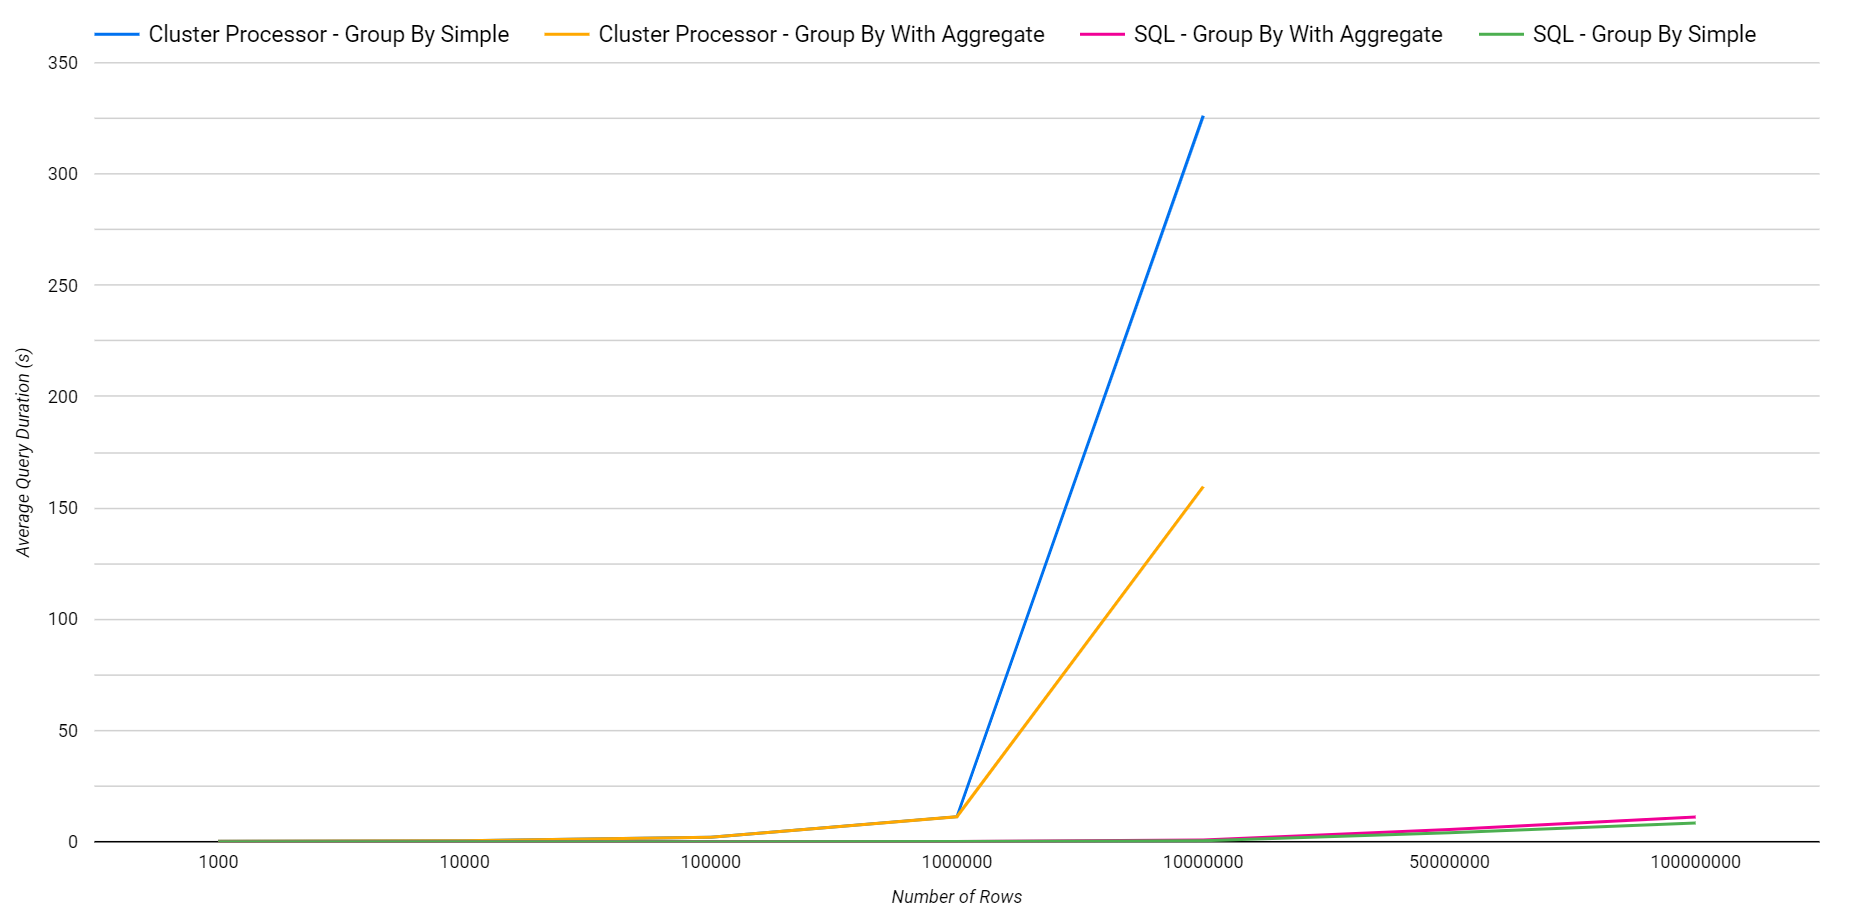
\includegraphics[width=0.8\linewidth]{chapters/diagrams/testing/group-by-1k-100m}
	\caption{SQL vs Cluster Processor - Group By Query Results}
	\label{fig:group-by-graph}
\end{figure}

\subsection{Analysis}
As the raw performance testing results show, a significant amount of optimisation would be required for the Cluster Processor solution to truly compete with SQL with regards to computation speed. In particular, the system appears to be weakest at transmitting raw data quickly across the network, as well as computing Group Bys quickly.

The main way the transmission format for results could be optimised is to ensure row is as small as possible. One potential way of doing this is to avoid sending type information with the value data, and use the header information to perform a conversion when the row is received, which would reduce the size of the row message. 

There are a number of ways in which Group By calculations could be optimised. Firstly, the same transmission format for sending results to the Python frontend is used by the workers for cross-communication. This means that any optimisations to the transmission format would also result in faster Group By computations. Another optimisation would be to reduce the amount of data that needs to be sent when workers cross-communicate. Currently, for simplicity, all data related to a given partition is sent between the workers, which results in a large amount of data being transferred across the network. It should be possible to partially perform the Group By operation for each partition on each worker, then finalise all partial results on the worker that actually holds the partition. This would significantly reduce the amount of data transferred across the network, and reduce the memory usage while computing the Group By.

\section{Level of Parallelisation}
This section will compare the performance of the Cluster Processor when the number of workers is varied, but the overall performance in terms of available resources is the same. The aim is to determine how changing the level of parallelisation in the cluster impacts the computation speed. 

In these tests the simple versions of the Select, Filter and Group By queries were executed, with a different range of rows depending on the test. See Appendix \ref{cha:testing-figs} for details of the queries that were executed. Figure \ref{fig:parallelisation-test-workers} shows the cluster layouts for each test case; the number of workers, and the resources available to each worker. As shown, the overall number of vCores and GB of memory available to the cluster is the same in each case.

Throughout all of these tests, the number of Cassandra nodes in the cluster remained consistent: 3 nodes, one placed on each Kubernetes node.

\begin{figure}[h]
	\centering
	\begin{tabular}{| c | c | c | c | c |}
		\hline
		\textbf{Workers} & \textbf{vCores} & \textbf{Worker Memory} & \textbf{Total vCores} & \textbf{Total Memory} \\ \hline
		2 & 3 & 9GB & 6 & 18GB \\ \hline
		3 & 2 & 6GB & 6 & 18GB \\ \hline
		6 & 1 & 3GB & 6 & 18GB \\ \hline
		9 & 0.666 & 2GB & 6 & 18GB \\ \hline
		12 & 0.5 & 1.5GB & 6 & 18GB \\ \hline
	\end{tabular}
	\caption{Parallelisation - Number of Workers and Resources}
	\label{fig:parallelisation-test-workers}
\end{figure}

\subsection{Select Query}
The results of this test are shown in Figure \ref{fig:select-simple-parallelisation-test}. Due to the same memory issue as in the SQL test, only 1000 to 100000 row tables were tested. The cluster layout with 3 nodes appears to execute around twice as fast across all data volumes. The other cluster layouts have similar execution times, with 12 nodes, the most parallelisation, running slowest by a small margin. Ultimately, this test is checking how fast each layout can pull data from Cassandra, and send it to the Orchestrator. It is likely that the extra overhead introduced by the higher levels of parallelisation slowed down data transfer, and there was no computation to perform which would benefit the increased number of nodes.

Interestingly, the 2 node cluster also performed slower than the 3 node cluster. This is likely to be because there was one less worker node than Cassandra node in this case, meaning some amount of latency was added to retrieve data from the Cassandra node without a co-located worker.

\begin{figure}[h]
	\centering
	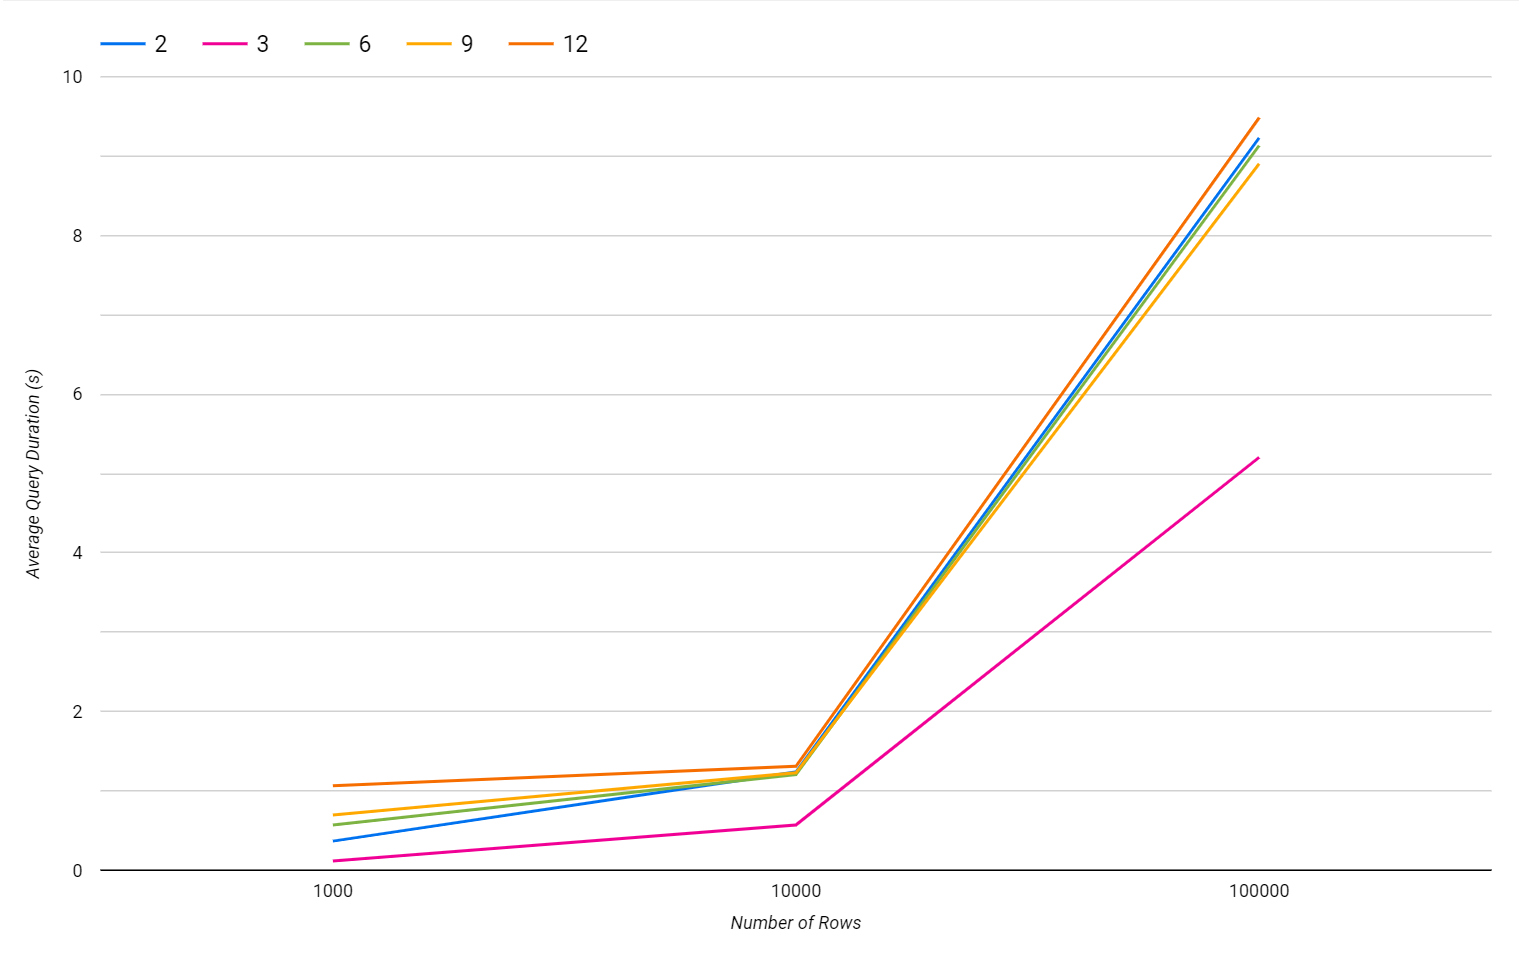
\includegraphics[width=0.8\linewidth]{chapters/diagrams/testing/select-simple-parallelisation-test}
	\caption{Parallelisation - Select Query Results}
	\label{fig:select-simple-parallelisation-test}
\end{figure}

\subsection{Filter Query}
The results of this test are shown in Figure \ref{fig:filter-simple-parallelisation-test}. At small numbers of rows, there is very little difference between each of the cluster layouts. However, an interesting trend appears as the number of rows increases above 100,000. The 3 node cluster is fastest until this point, but is then overtaken by the 9 node cluster at 1 million.

To investigate this trend further, the test was also run for all cluster layouts at 10 million rows, shown in Figure \ref{fig:filter-simple-parallelisation-10m}. At this number of rows, the layouts with 6, 9 and 12 nodes are all faster than the 3 node cluster, with 9 nodes appearing to be the optimal level of parallelisation. This shows that as the amount of work to perform increases, the increased level of parallelisation becomes a benefit, resulting in faster computation times. The fact that 12 nodes is slower than 9 nodes at 10 million rows suggests that there is an optimal point in terms of maximising parallelisation, without introducing too much overhead from the number of nodes.

\begin{figure}[h]
	\centering
	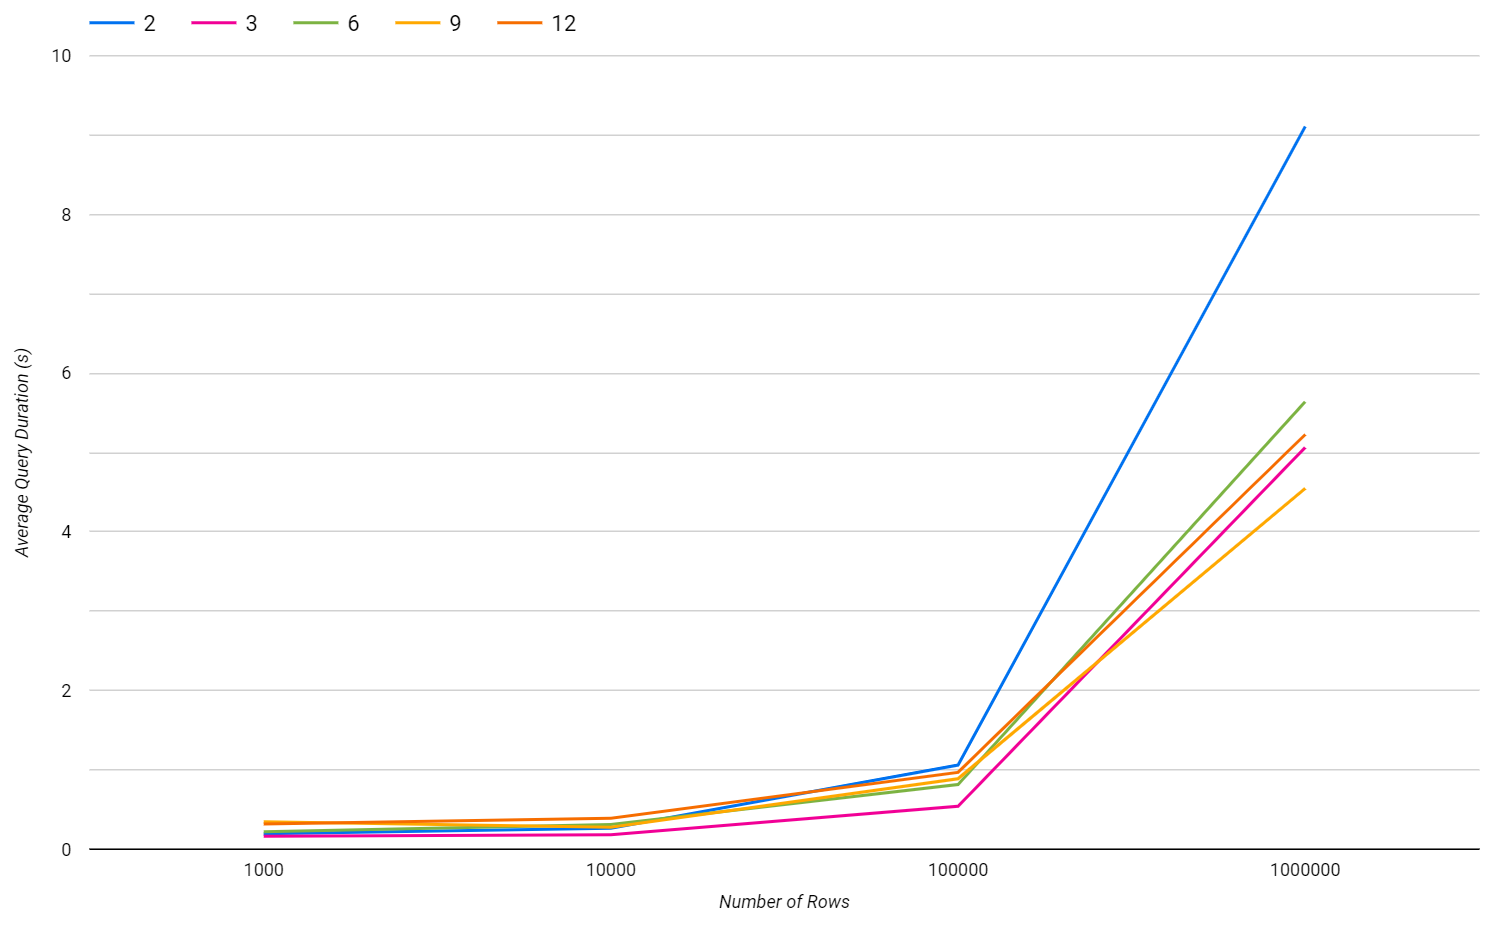
\includegraphics[width=0.8\linewidth]{chapters/diagrams/testing/filter-simple-parallelisation-test}
	\caption{Parallelisation - Filter Query Results}
	\label{fig:filter-simple-parallelisation-test}
\end{figure}

\begin{figure}[h]
	\centering
	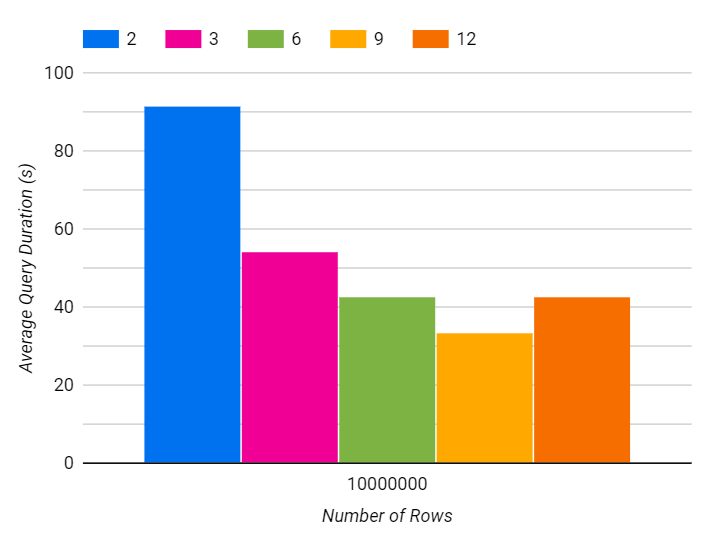
\includegraphics[width=0.4\linewidth]{chapters/diagrams/testing/filter-simple-parallelisation-10m}
	\caption{Parallelisation - Filter Query Results, 10 Million Rows}
	\label{fig:filter-simple-parallelisation-10m}
\end{figure}

\subsection{Group By Query}
The results of this test are shown in Figure \ref{fig:group-by-simple-parallelisation-test}. These results again suggest that there is a balancing point for the level of parallelisation. The 3 node cluster is consistently faster than all other cluster layouts. The 6, 9 and 12 cluster layouts are likely to be slower because increasing the level of parallelisation will result in higher amounts of cross-communication, and network transfer is one of the slowest areas, as identified in the SQL test.

Interestingly, the 2 node cluster is second fastest until 1 million rows, when its performance significantly reduces. This is likely to be because the increased memory demands on each node caused by having fewer worker nodes resulted in some data being spilled to disk, which results in reduced query performance.

\begin{figure}[h]
	\centering
	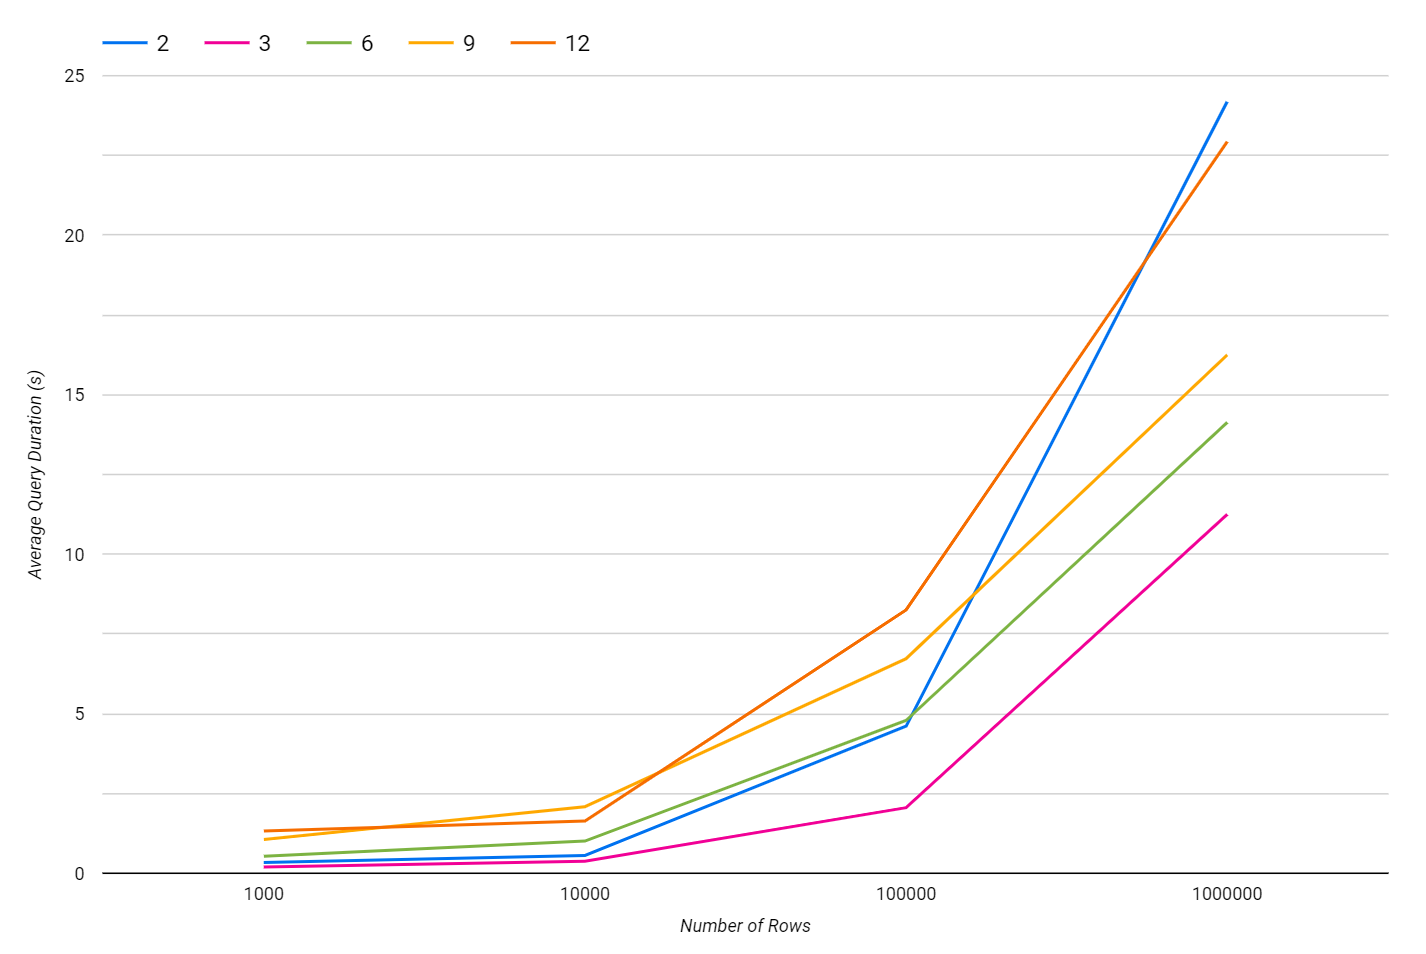
\includegraphics[width=0.8\linewidth]{chapters/diagrams/testing/group-by-simple-parallelisation-test}
	\caption{Parallelisation - Group By Query Results}
	\label{fig:group-by-simple-parallelisation-test}
\end{figure}

\subsection{Analysis}
Overall, the outcomes of this test show that there is no clear solution to the number of nodes in the cluster. As a general rule, matching the number of workers to the number of Cassandra nodes in the cluster will result in good performance, but the Filter test also shows that increasing the level of parallelisation can result in better performance for the same resources at larger query sizes. Solutions to this problem depend entirely on the queries being run, and the data volumes the queries are applied to. There is an opportunity for further research designing a system that can analyse the queries being executed, and adjust the cluster layout to match the requirements of those queries.

\section{Autoscaling}
This section will compare computation speed of the Cluster Processor when the overall performance is reduced. This test is motivated by the autoscaling feature present in many managed Kubernetes services, including Azure Kubernetes Service \todo{reference}. This feature continually analyses the load of the Kubernetes cluster, and increases or decreases the number of physical nodes based on current demand. By doing this, applications with fluctating levels of demand are able to save costs by reducing the number of machines they pay for in periods of low demand.

While the Cluster Processor is not currently implemented in a way that supports autoscaling, this test is performed to identify how effective autoscaling would be on this solution. In these tests the simple versions of the Select, Filter and Group By queries were executed, with a different range of rows depending on the test. Figure \ref{fig:autoscale-test-workers} shows the cluster layouts for each test case; the number of workers, and the resources available to each worker. Each cluster layout has one less worker, and 33\% less resources available.

Throughout all of these tests, the number of Cassandra nodes in the cluster remained consistent: 3 nodes, one placed on each Kubernetes node.

\begin{figure}[h]
	\centering
	\begin{tabular}{| c | c | c | c | c |}
		\hline
		\textbf{Workers} & \textbf{vCores} & \textbf{Worker Memory} & \textbf{Total vCores} & \textbf{Total Memory} \\ \hline
		3 & 2 & 6GB & 6 & 18GB \\ \hline
		2 & 2 & 6GB & 4 & 12GB \\ \hline
		1 & 2 & 6GB & 2 & 6GB \\ \hline
	\end{tabular}
	\caption{Autoscaling - Number of Workers and Resources}
	\label{fig:autoscale-test-workers}
\end{figure}

\subsection{Select Query}
The results of this test are shown in Figure \ref{fig:select-simple-autoscale-test}. As expected, the query performance decreases as the number of workers decreases. However, at 1000 rows the difference between 3 workers and 1 worker is around 0.3s, and at 10000 rows it is 0.9s

\begin{figure}[h]
	\centering
	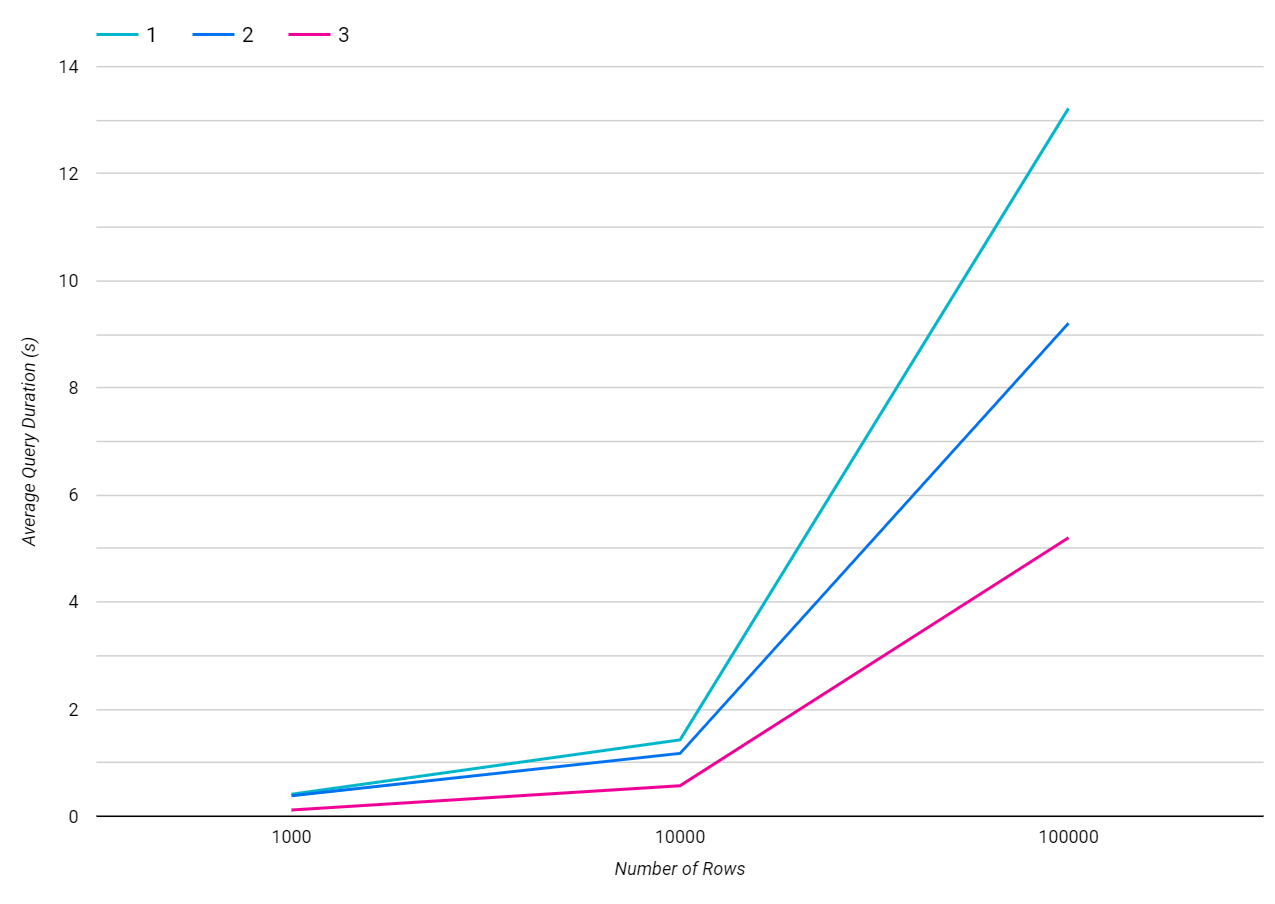
\includegraphics[width=0.8\linewidth]{chapters/diagrams/testing/select-simple-autoscale-test}
	\caption{Autoscaling - Select Query Results}
	\label{fig:select-simple-autoscale-test}
\end{figure}

\subsection{Filter Query}
The results of this test are shown in Figure \ref{fig:filter-simple-autoscale-test}. As before, the query performance decreases as the number of workers decreases. However, at small data volumes the difference between 1 and 3 workers is even smaller than in the Select test. The difference between 1 and 3 workers is 0.08s at 1000 rows, 0.2s at 10000 rows, and 1.1s at 100,000 rows.

\begin{figure}[h]
	\centering
	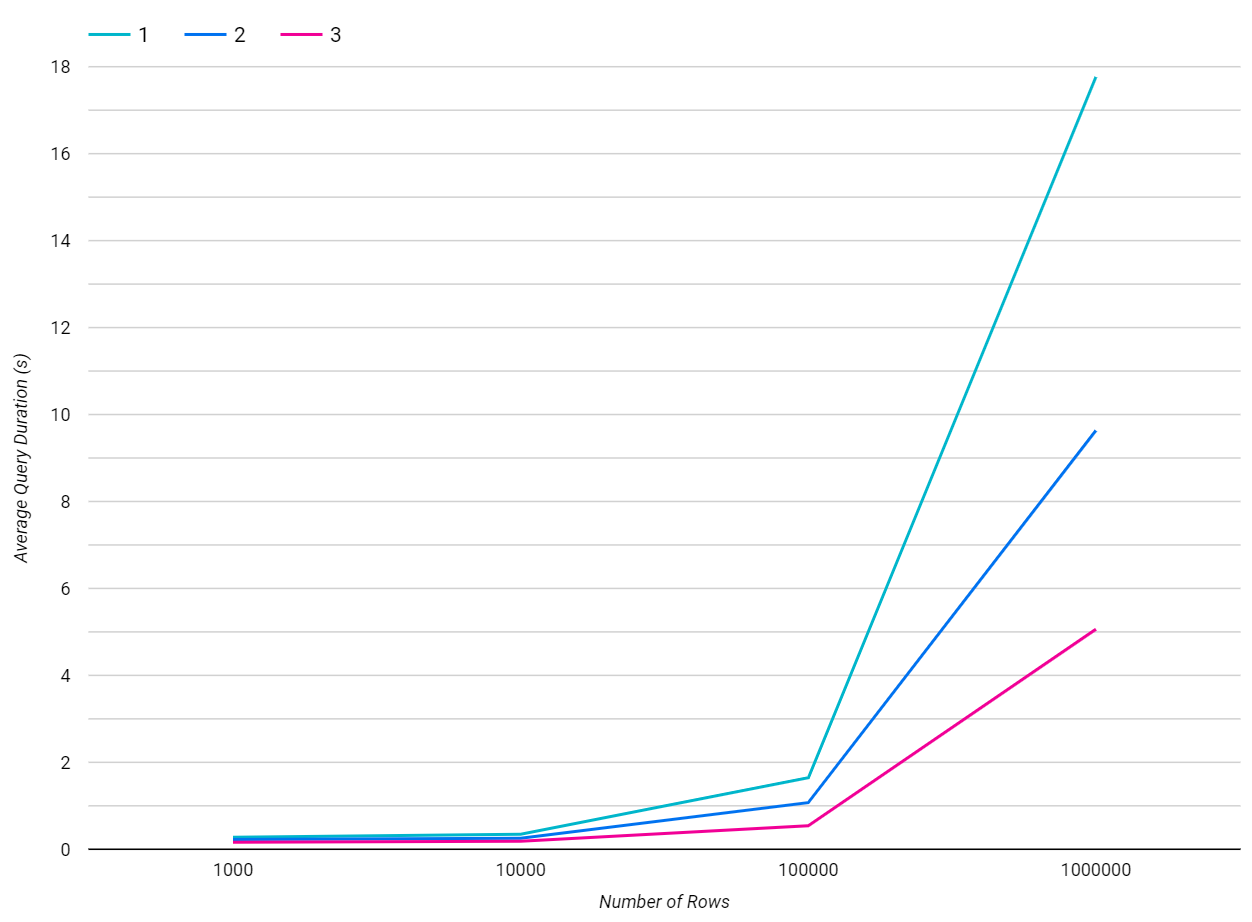
\includegraphics[width=0.8\linewidth]{chapters/diagrams/testing/filter-simple-autoscale-test}
	\caption{Autoscaling - Filter Query Results}
	\label{fig:filter-simple-autoscale-test}
\end{figure}

\subsection{Group By Query}
The results of this test are shown in Figure \ref{fig:group-by-simple-autoscale-test}. At 1000 and 10000 rows, there is effectively no difference between the three cluster layouts, and at 100000 rows the 1 node cluster is the fastest by 0.5s on average. Once the data volume increases to 1 million rows, the 3 node cluster is significantly faster than the other two layouts. However, these results suggest that, at very small data volumes, it is faster to perform all of the computation on a single node. This is because it prevents the need for the workers to cross-communicate, and if all data can be kept in memory, the computation will be performed significantly faster.

\begin{figure}[h]
	\centering
	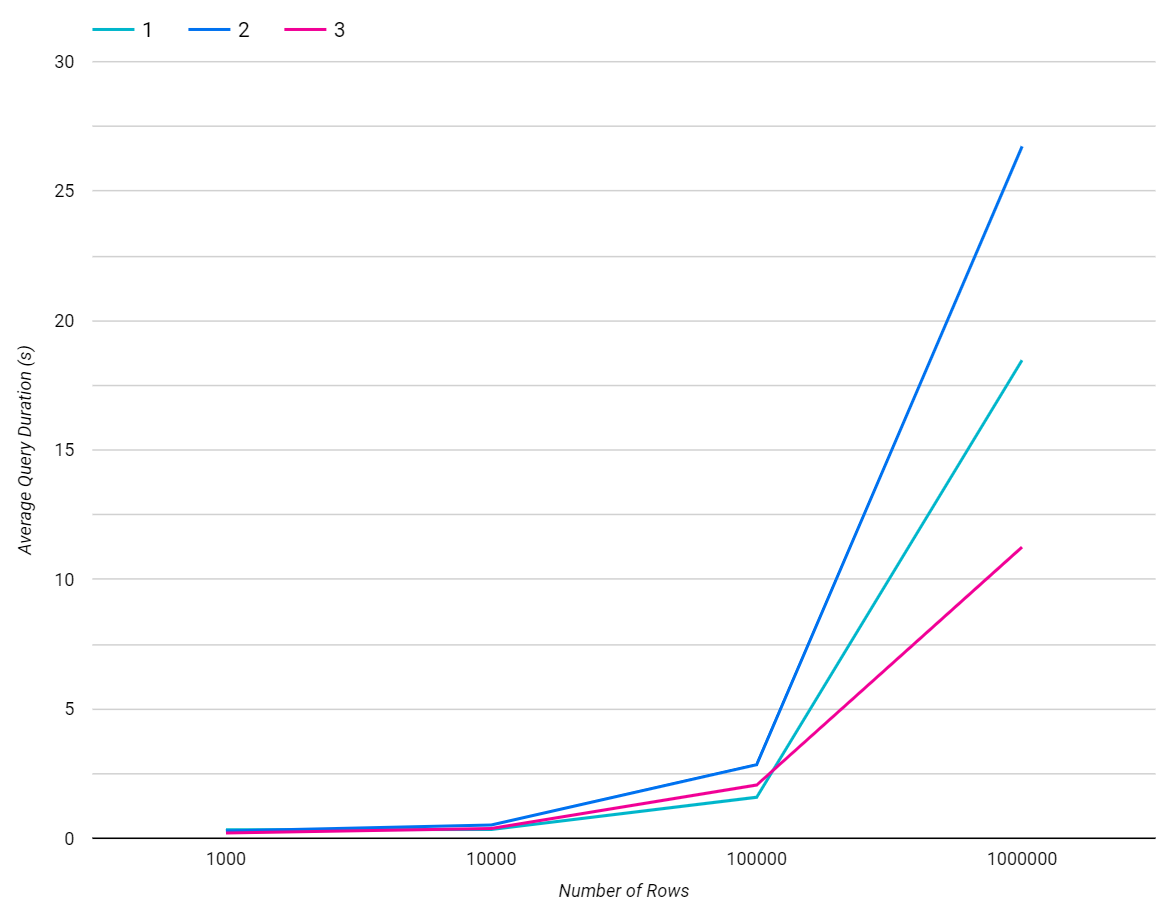
\includegraphics[width=0.8\linewidth]{chapters/diagrams/testing/group-by-simple-autoscale-test}
	\caption{Autoscaling - Group By Query Results}
	\label{fig:group-by-simple-autoscale-test}
\end{figure}

\subsection{Analysis}
The outcomes of this test show that it is effective to reduce the cluster size if the data volumes are small. The time difference between the smallest and largest cluster typically less than a second when operating on less than 1 million rows. This is insignificant for most use cases, and if a time-critical system was reliant on querying this small amount of data, a more typical solution like SQL would be better suited to solve the problem regardless.
